% !TeX root = ../main.tex

\chapter{基于双层缓存的优先经验重放算法}

\section{强化学习中的经验回放}

第一章研究现状介绍过经验重放(Experience Replay, ER)机制可以有效地提
高数据样本的使用效率,还可以打破数据之间的相关性,避免深度神经网络训练 因数据的连续性导致的不稳定性。而为了更高效地利用有用的经验,人们改变了 随机经验重放的方法,提出了改进的优先经验重放。在优先经验重放方法中,通 常会为记忆库中的经验定义它们的优先级,改变每条经验被重放的概率,让那些 重要的、优秀的或对学习有利的经验更有可能被学习。而在各种优先经验重放算 法中,目前最流行的一种是由 DeepMind 团队在深度 Q 网络(Deep Q-Network, DQN)算法的基础上提出的优先经验重放(Prioritized Experience Replay, PER)算 法。

% The Prioritized Experience Replay (PER) method has achieved good results in reinforcement learning, but it still has many limitations, including too much repetitive experience replay of outdated memories and poor coverage of the entire sample space. However, existing works have not paid much attention to this issue. We provide empirical insight that double layer replay buffer can help learn more important experiences which help improve the efficiency of reinforcement learning, while addressing the aforementioned limitations. In this work, to alleviate these limitations, we design a double layer experience replay mechanism. We add a second layer replay buffer based on the usual experience replay method, and extract samples from the experience pool in real time and add them to the second layer replay buffer. The samples in both of the two buffers are then mixed for policy optimization. We show that our method does provide near-ideal prioritized sampling distributions. We conduct experiments to demonstrate the effectiveness of our method.

优先经验重放(PER)方法在强化学习中取得了很好的效果,但它仍有很多局限性,包括对过期记忆的重复经验重放太多,对整个样本空间的覆盖率不高。然而,现有的工作并没有对这个问题给予太多的关注。我们提供了经验性的见解,即双层重放缓冲区可以帮助学习更多的重要经验,这有助于提高强化学习的效率,同时解决上述的局限性。在这项工作中,为了缓解这些限制,我们设计了一个双层经验重放机制。我们在通常的经验重放方法的基础上增加了第二层重放缓冲区,并从经验池中实时提取样本,并将其加入第二层重放缓冲区。然后,这两个缓冲区中的样本被混合起来进行策略优化。我们表明,我们的方法确实提供了接近理想的优先采样分布。我们进行了实验来证明我们方法的有效性。

\section{Introduction}

% In recent years, reinforcement learning (RL) has achieved remarkable results in a wide range of fields. However, reinforcement learning still faces challenges in practical application. The most obvious one is the sample efficiency problem. Although reinforcement learning has achieved excellent results in some fields, it often relies on huge training samples, which is not practical in the real world. Since there is no trial-and-error cost in a virtual simulation environment, algorithms are free to perform exploratory learning and thus learn strategies that can circumvent wrong decisions. However, in the real world, where much trial-and-error implies huge costs, it becomes a major challenge to learn decisions that can circumvent errors within limited training samples.

近年来,强化学习(RL)在广泛的领域取得了显著的成果。然而,强化学习在实际应用中仍然面临挑战。其中最明显的是样本效率问题。尽管强化学习在一些领域取得了卓越的成果,但它往往依赖于巨大的训练样本,这在现实世界中并不实用。由于在虚拟的模拟环境中没有试错成本,算法可以自由地进行探索性学习,从而学习可以规避错误决策的策略。然而,在现实世界中,大量的试错意味着巨大的成本,如何在有限的训练样本中学习能够规避错误的决策成为一个重大挑战。

% Experience Replay (ER) ~\cite{lin1992self} has been a popular method for training large-scale reinforcement learning scenarioes ~\cite{degris2012continuous, vincent2018introrl}. In experience replay, the visited experiences are stored in a buffer, and at each time step, a batch of experiences are sampled to update the training parameters in the value function or policy. Experience shows that such an approach can be effective in stabilizing training and improving the sampling efficiency of deep RL algorithms. Several subsequent works have proposed different variants to improve it ~\cite{schaul2016prioritized,junhyuk2018selfil,horgan2018distributed,sun2020er}. The most relevant to our work is the prioritized experience replay (PER) ~\cite{schaul2016prioritized}. PER is a prioritized extraction method when sampling past trajectories from a experience pool, which attempts to improve the vanilla experience replay method by sampling those visited experiences in proportion to the absolute Temporal Difference (TD) errors. The reason for the improvement of PER over the traditional experience replay method is that randomly extracted experience ignores some important experiences. Just like the human brain, there exist memories that are more important and worthy of being learned. The effect of the PER method is to be able to learn the important experiences better, allowing the algorithm to converge faster and better.

Experience Replay(ER)\cite{lin1992self}一直是训练大规模强化学习场景的流行方法~cite{degris2012continuous, vincent2018introrl}。在经验回放中,访问过的经验被存储在一个缓冲区中,在每个时间步骤中,对一批经验进行采样,以更新价值函数或策略中的训练参数。经验表明,这种方法可以有效地稳定训练并提高深度RL算法的采样效率。随后的几项工作提出了不同的变体来改善它\cite{schaul2016prioritized,junhyuk2018selfil,horgan2018distributed,Sun2020er}。与我们的工作最相关的是优先经验回放(PER)\cite{schaul2016prioritized}。PER是一种从经验池中抽取过去轨迹时的优先提取方法,它试图通过按照绝对时差(TD)误差的比例抽取那些访问过的经验来改进香草式经验重放方法。PER比传统的经验重放方法有所改进的原因是,随机提取的经验忽略了一些重要的经验。就像人的大脑一样,存在着一些更重要的、值得学习的记忆。PER方法的效果是能够更好地学习重要的经验,使算法能够更快更好地收敛。

% PER makes replay more efficient than pure random sample replay by prioritizing experience. The ideal approach is to count the number of times the agent learns from transitions in the current state, but this metric is actually not easy to obtain. A more feasible way is to calculate the TD-error of each transition. If the TD-error is larger, it means that there is still a lot of room for improvement in our prediction accuracy, and the more this sample needs to be learned, that is, the higher the priority is.

PER通过优先考虑经验,使重放比纯随机样本重放更有效率。理想的方法是计算代理从当前状态的过渡中学习的次数,但这个指标实际上不容易获得。一个更可行的方法是计算每个过渡的TD-误差。如果TD-误差比较大,说明我们的预测精度还有很大的提升空间,这个样本需要学习的次数越多,也就是说,优先级越高。

% Despite the mentioned enhancements, the PER approach still has some problems: 1) In order to avoid the expensive cost of scanning the entire experience pool, only the TD-error value of the replayed transition will be updated, which will result in the transitions with small TD-error seen for the first time and will not be replayed for a long time; 2) TD-error is very sensitive to noise, and it is easy to add estimation errors due to noise; 3) High TD-error and frequent replays can cause overfitting due to loss of diversity.

尽管有上述改进,PER方法仍然存在一些问题:1)为了避免扫描整个经验库的昂贵成本,只有重放的过渡的TD-误差值会被更新,这将导致第一次看到的TD-误差小的过渡不会被长时间重放;2)TD-误差对噪声非常敏感,很容易因噪声而增加估计误差;3)高TD-误差和频繁重放会因损失多样性而导致过拟合。

% In fact, PER only performs priority assignment on the replay buffer composed of visited states. Compared with the entire state space, all training samples may only constitute a small subset, so PER is only in a local small space. After changing the sample distribution, the priority distribution in the global sense cannot be achieved, and the actual implementation is far from its concept.

事实上,PER只对由访问过的状态组成的重放缓冲区进行优先级分配。与整个状态空间相比,所有的训练样本可能只构成一个小的子集,所以PER只是在一个局部的小空间。在改变了样本分布后,全局意义上的优先权分配就无法实现,实际的实现与它的概念相差甚远。

% In this paper, we design a double layer experience replay mechanism to solve the limitations mentioned above. Like the usual experience replay approach, it first stores the observed samples in the
% experience replay pool. But the difference is that  a second replay buffer is added afterwards for prioritizing the samples. The motivation for this is that we consider that humans do not fully prioritize all experiences when learning from experience, but only partially select important experiences to be learned first. We also set parameters to determine the size of the second layer buffer to dynamically adjust the degree of priority experience replay.

在本文中,我们设计了一种双层经验重放机制来解决上述的限制。与通常的经验重放方法一样,它首先将观察到的样本存储在
经验重放池。但不同的是,之后增加了第二个重放缓冲区,以确定样本的优先次序。这样做的动机是,我们认为人类在从经验中学习时,不会完全优先考虑所有的经验,而只是部分地选择重要的经验来先学习。我们还设置了一些参数来决定第二层缓冲区的大小,以动态地调整优先经验重放的程度。

\section{Related Work} \label{sec:Background}

% In this section, we firstly review basic concepts in RL. Then we briefly introduce the prioritized ER method, which will be examined in-depth in the next section. We conclude this section by discussing a classic model based reinforcement learning architecture called Dyna~\cite{sutton1991integrated} and its recent variants, which are most relevant to our work. 

在本节中,我们首先回顾RL的基本概念。然后,我们简要介绍了优先考虑的ER方法,这将在下一节深入研究。在这一节的最后,我们讨论了一个经典的基于模型的强化学习架构,即Dyna\cite{sutton1991integrated}及其最近的变体,这与我们的工作最为相关。

% \begin{figure*}
%     \centering
%     \subfigure[Cliff Walking Environment]{
%         \centering
%         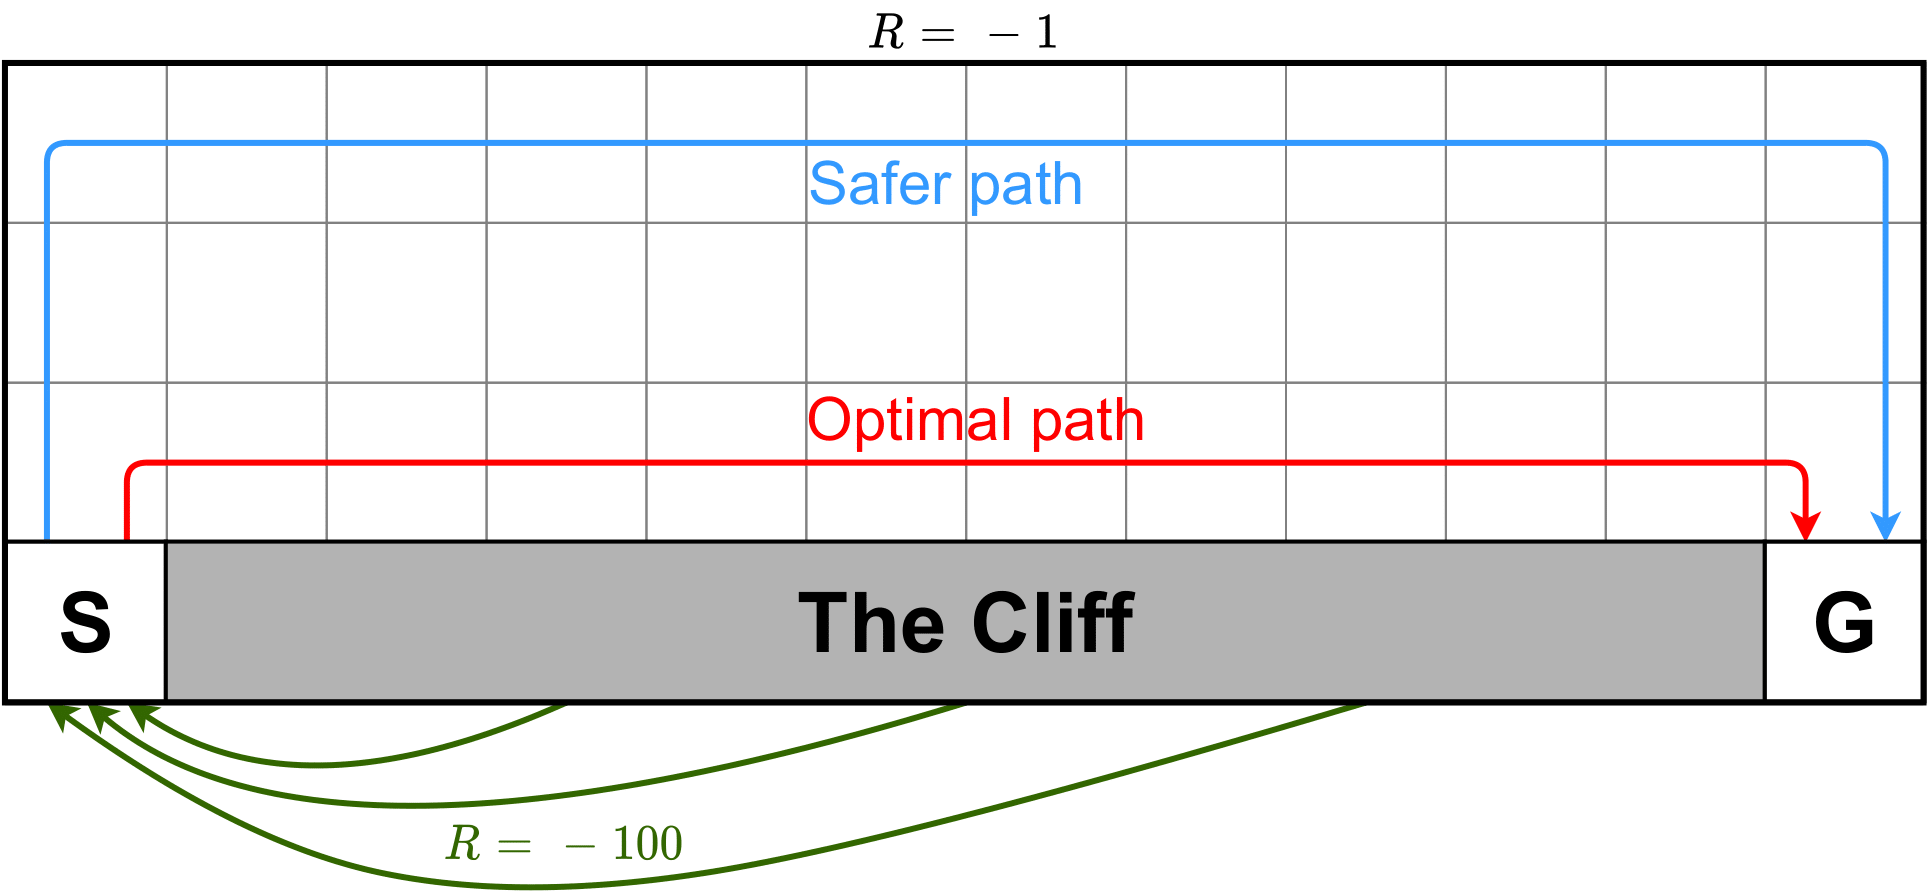
\includegraphics[width=0.45\textwidth]{imgs/cliff-env.png}
%         \label{fig:cliff-env}
%     }
%     \hspace{0.5cm}
%     \subfigure[The effect of rollout dropout]{
%         \centering
%         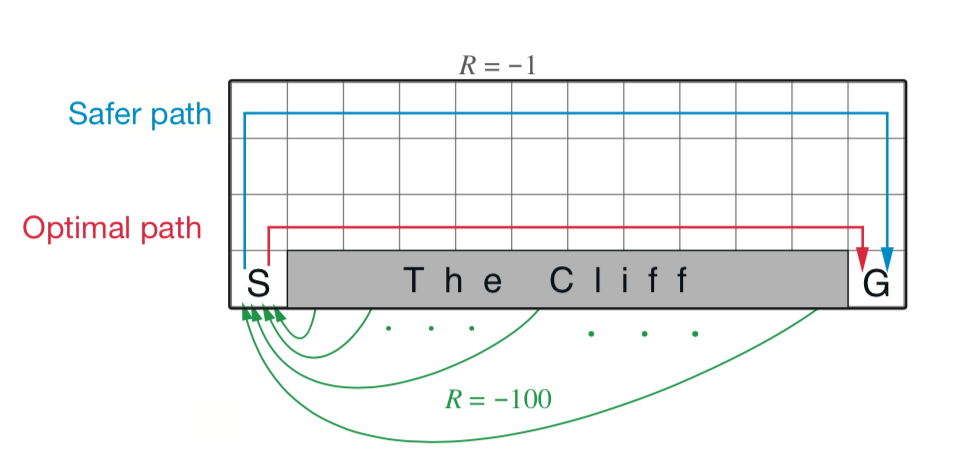
\includegraphics[width=0.45\textwidth]{imgs/cliffwalking.png}
%         \label{fig:cliff-dis}
%     }
%     \caption{(a) The Cliff Walking Env consists of $4\times 12$ squares, where the bottom left corner is the start point, the bottom right corner is the goal point, the remaining squares in the bottom row are cliff, and the rest of the squares are normal states. When agent enters the cliff, it gets a reward of $-100$ and immediately ends the current episode, while in all other states, it gets a reward of $-1$; (b) The horizontal axis is the number of training steps, and the vertical axis indicates the Euclidean Distance of the agent from the cliff at the corresponding moment. Solid curves indicate the mean of all trials with different seeds. Shaded regions correspond to standard deviation among trials.}
% \end{figure*}

% Reinforcement learning (RL) algorithms are commonly divided into two categories: model-free RL and model-based RL. Model-free RL methods learn policy directly from observed samples in the real environment, while model-based RL approaches build approximate predictive models of the environment and then derive policy from samples generated by the predictive model \cite{chen2015reinforcement,polydoros2017survey}. In recent years, reinforcement learning has achieved remarkable results in a wide range of areas, including simulated control problems \cite{schulman2015high,lillicrap2015continuous,levine2016end}, outperforming human performances on Go and games \cite{mnih2015human,silver2016mastering}. However, these results are mostly achieved by model-free reinforcement learning algorithms that rely on a large number of real-world environmental samples, and therefore these algorithms are often limited to a simulated environment when deploying applications. In contrast, model-based methods have shown promising ability in reducing the sample complexity \cite{deisenroth2013survey,berkenkamp2017safe}. Previous works \cite{levine2016end,Chua2018DeepModels,janner2019trust} have empirically shown significant improvements in sample efficiency.

强化学习(RL)算法通常分为两类:无模型RL和基于模型RL。无模型RL方法直接从真实环境中观察到的样本中学习策略,而基于模型的RL方法则是建立环境的近似预测模型,然后从预测模型产生的样本中得出策略 (\cite{chen2015reinforcement,polydoros2017survey}。近年来,强化学习在很多领域取得了令人瞩目的成果,包括模拟控制问题 (\cite{schulman2015high,lillicrap2015continuous,levine2016end},超越人类在围棋和游戏上的表现 (\cite{mnih2015human,Silver2016mastering}。然而,这些结果大多是由无模型的强化学习算法实现的,这些算法依赖于大量的真实世界环境样本,因此这些算法在部署应用时往往被限制在模拟环境中。相比之下,基于模型的方法在降低样本复杂度方面表现出很好的能力 (\cite{deisenroth2013survey,berkenkamp2017safe}。以前的工作\cite{levine2016end,Chua2018DeepModels,janner2019trust}在经验上显示了样本效率的显著提高。


% Model-based reinforcement learning is a powerful tool to improve sample efficiency by interacting with the simulated environment. DeepPILCO method \cite{gal2016improving} enables modeling more complex environments by introducing Bayesian Neural Network (BNN) with high-capacity function approximators for neural networks \cite{blundell2015weight,mackay1995bayesian}. Model ensemble method \cite{kurutach2018model} is further introduced to comprehensively capture the uncertainty in the environment \cite{malik2019calibrated}. In this paper, we adopt the model ensemble approach and combine it with our designed dropout mechanism to achieve controllability of performance and robustness. However, all of these model-based methods suffer from model bias, resulting in bad decision policies. STEVE method \cite{buckman2018sample} tries to solve this problem by dynamically interpolating the length of rollouts for better performance. MBPO method \cite{janner2019trust} starts from real states and only performs short length rollouts in planning, which can effectively avoid the accumulated errors. With a model, an agent has more flexibility to sample hypothetical experiences. We consider a one-step model which maps a state-action pair to its possible next state and reward: $M:sxa$. We build on the Dyna formalism~\cite{sutton1991integrated} for MBRL, and more specifically, the proposed Dyna Style MBRL as shown in Algorithm~\ref{algo:mbrl}. Dyna Style MBRL is a very general model based reinforcement learning framework on which to build algorithms that can be easily extended to a variety of specific improvement methods.

基于模型的强化学习是一个强大的工具,通过与模拟环境的互动来提高采样效率。DeepPILCO方法\cite{gal2016improving}通过引入贝叶斯神经网络(BNN)与神经网络的高容量函数近似器,实现了对更复杂环境的建模\cite{blundell2015weight,mackay1995bayesian}。进一步引入了模型集合方法 \cite{kurutach2018model}来全面捕捉环境的不确定性 \cite{malik2019calibrated}。在本文中,我们采用了模型集合方法,并将其与我们设计的辍学机制相结合,以实现性能的可控性和鲁棒性。然而,所有这些基于模型的方法都存在着模型偏差,导致决策策略不好。STEVE方法\cite{buckman2018sample}试图通过动态插值退出的长度来解决这个问题,以获得更好的性能。MBPO method \cite{janner2019trust}从真实状态出发,在规划中只执行短长度的滚动,这样可以有效避免累积的错误。有了模型,代理人就有了更大的灵活性,可以对假设的经验进行采样。我们考虑一个单步模型,它将一个状态-行动对映射到其可能的下一个状态和奖励:$M:sxa$。我们建立在Dyna形式主义\cite{sutton1991integrated}的MBRL上,更具体地说,就是算法\ref{algo:mbrl}中提出的Dyna风格的MBRL。Dyna Style MBRL是一个非常通用的基于模型的强化学习框架,在此基础上建立的算法可以很容易地扩展到各种具体的改进方法。

% Experience Replay is critical when using neural networks to estimate $Q_\theta$, as used in DQN~\cite{mnih2015human}, both to stabilize and speed up learning. ER method uniformly samples a mini-batch of experiences from those visited ones in the form of $(s_t, a_t, s_{t+1}, r_{t+1})$ to update neural network parameters. Prioritized ER~\cite{schaul2016prioritized} improves upon it by prioritized sampling experiences, where the probability of sampling a certain experience is proportional to its TD error magnitude, i.e., $p(s_t, a_t, s_{t+1}, r_{t+1})\propto |\delta_{t}|$. However, the underlying theoretical mechanism behind this method is still not well understood.

当使用神经网络来估计$Q_\theta$时,经验重放是至关重要的,就像在DQN\cite{mnih2015human}中使用的那样,既能稳定又能加快学习速度。ER方法以$(s_t, a_t, s_{t+1}, r_{t+1})$的形式从那些访问过的经验中均匀地抽出一个小批,以更新神经网络参数。Prioritized ER\cite{schaul2016prioritized}通过优先抽样经验来改进它,其中抽样某个经验的概率与它的TD误差大小成正比,即$p(s_t, a_t, s_{t+1}, r_{t+1})propto |\delta_{t}|$。然而,这种方法背后的基本理论机制仍然没有得到很好的理解。

\section{DPER Method}

\subsection{A Motivating Example}

% In order to understand the potential benefits of double layer experience replay, we introduce a Cliff Walking environment (described in Figure \ref{fig:cliff-env}). Obviously, there is an optimal path, as shown by the red line in the figure. However, this optimal path is also the most dangerous one. If the algorithm is not efficient in early stage, it may accidentally enter the cliff from the optimal path at any time, resulting in a large penalty, thus affecting the convergence of the algorithm, so the algorithm with better robustness can perform better in the Cliff Walking environment.

% We use the Policy Gradient (PG) algorithm and design a variant that would dropout some rollout samples while conducting comparative experiments in the Cliff Walking environment. As shown in Figure \ref{fig:cliff-dis}, the agent in the original PG algorithm tends to explore from a safe path away from the cliff until it gets sufficient information to slowly approach the optimal path. In contrast, the PG algorithm with double layer experience replay can learn more quickly and can more confidently approach the danger region earlier and thus converge to the optimal path better. The statistical results show that the policies trained with the double layer experience replay method fall into the cliff region less often and exhibit better robustness during evaluation.

% Table \ref{tab:cliff-stats} shows the evaluation statistical results of the policy gradient using single or double layer replay buffer in the CliffWalking environment. The metrics are the probability of falling into the cliff area, and the average return. Each run of the experiment consists of 3 sets of seeds, and each experiment takes 2000 steps. It can be seen that when the double layer replay buffer is used, the algorithm performs better than the case of single layer replay buffer. This motivation experiment gives us an inspiration to design our algorithm.

为了理解双层经验重放的潜在好处,我们引入了一个悬崖行走环境(如图\ref{fig:cliff-env}所述)。很明显,有一条最优路径,如图中的红线所示。然而,这条最优路径也是最危险的路径。如果算法在早期阶段效率不高,随时可能不小心从最优路径进入悬崖,造成较大的惩罚,从而影响算法的收敛性,所以具有较好鲁棒性的算法在悬崖行走环境中可以表现得更好。

我们使用政策梯度(PG)算法,并设计了一个变体,在悬崖行走环境中进行对比实验时,会放弃一些滚动样本。如图所示,原始PG算法中的代理人倾向于从远离悬崖的安全路径进行探索,直到它获得足够的信息来慢慢接近最优路径。相比之下,具有双层经验重放的PG算法能够更快地学习,并且能够更有把握地提前接近危险区域,从而更好地收敛到最优路径。统计结果表明,用双层经验重放法训练的策略落入悬崖区的次数较少,在评估过程中表现出更好的稳健性。

表\ref{tab:cliff-stats}显示了在CliffWalking环境下使用单层或双层重放缓冲区的策略梯度的评估统计结果。这些指标是落入悬崖区的概率,以及平均回报率。每次实验的运行由3组种子组成,每次实验需要2000步。可以看出,当使用双层重放缓冲器时,该算法的表现比单层重放缓冲器的情况要好。这一激励性实验给了我们设计算法的灵感。

\subsection{Double Layer Experience Replay}

% In this subsection, we will introduce the Double Layer Experience Replay method and how it can help improve learning efficiency of Reinforcement Learning.

% We firstly train a model based on the environment data, i.e., $\mathcal{D}_{\text{env}}$. After obtaining the model, we first generate a certain amount of samples to fill in the multi-layer batch, first take out hypothetical samples with large deviations for learning, and then directly give priority to infer and learn in the direction that may have large deviations to make up for the shortcomings of the agent policy, followed by regular learning. With the idea of Dyna-style RL, we continually transmit the collected real samples to the model for further optimization in the policy optimization cycle, which enables the model to provide simulation samples for the framework more efficiently and accurately. We also use the model ensemble approach in order to capture the uncertainty in environment.

% The algorithmic framework maintains two buffers: the first layer experience replay buffer which stores general transition samples (the form of $(s_t, a_t, s_{t+1}, r_{t+1})$) and the second layer experience replay buffer which stores the prioritized transition samples. At each time step $t$, a real experience $(s_t, a_t, s_{t+1}, r_{t+1})$ is collected and stored into the first layer experience replay buffer. Then the priority process starts to prioritize the samples and store them into the second layer experience replay buffer. A hypothetical experience is obtained by first selecting a state $s$ from the experience replay buffer (as shown in Figure \ref{fig:algo-structure}), then selecting an action $a$ according to the current policy, and then querying the model to get the next state $s'$ and reward $r$ to form an experience $(s, a, s', r)$. These hypothetical transitions are combined with real experiences into a single replay buffer to update the training parameters. The updates performed before taking the next action, are called \emph{planning updates}~\cite{sutton2018intro}, as they improve the action-value estimates---and so the policy---using a model. The choice of pairing states with on-policy actions to form hypothetical experiences has been reported to be beneficial~\cite{gu2016continuous,yangchen2018rem,janner2019trustmodel}.

在本小节中,我们将介绍双层经验重放法以及它如何帮助提高强化学习的学习效率。

我们首先根据环境数据训练一个模型,即$\mathcal{D}_{text{env}}$。得到模型后,我们先生成一定量的样本填充到多层批处理中,先取出偏差较大的假设样本进行学习,然后直接优先推断并学习可能存在较大偏差的方向,以弥补代理策略的不足,接着进行常规学习。利用Dyna式RL的思想,我们在策略优化周期中不断将收集到的真实样本传输给模型进行进一步优化,这使得模型能够更高效、更准确地为框架提供模拟样本。我们还使用了模型集合的方法,以捕捉环境中的不确定性。

该算法框架保持两个缓冲区:第一层经验重放缓冲区,存储一般的过渡样本(形式为$(s_t, a_t, s_{t+1}, r_{t+1})$);第二层经验重放缓冲区,存储优先级的过渡样本。在每个时间步长$t$,一个真实的经验$(s_t, a_t, s_{t+1}, r_{t+1})$被收集并存储到第一层经验回放缓冲区。然后,优先级过程开始对样本进行优先排序,并将其存储到第二层经验重放缓冲区。一个假设的经验是通过首先从经验回放缓冲器中选择一个状态$s$(如图\ref{fig:algo-structure}所示),然后根据当前策略选择一个行动$a$,然后查询模型以获得下一个状态$s'$和奖励$r$,形成一个经验$(s, a, s', r)$。这些假想的过渡与真实的经验结合到一个重放缓冲区,以更新训练参数。在采取下一个行动之前进行的更新,被称为\emph{规划更新}~\cite{sutton2018intro},因为它们改善了行动价值的估计---因此也改善了政策---使用模型。据报道,选择将状态与政策上的行动配对,形成假设的经验是有益的\cite{gu2016continuous,yangchen2018rem,janner2019trustmodel}。

% Specifically, the scale is controlled by the parameter $\alpha$: the first $\alpha$ scale samples are planned for prioritized experience replay, and the latter $(1-\alpha)$ scale samples are used for regular learning. Then we fill the prioritized samples into the second layer buffer, and then correct the sample distribution through importance sampling in the buffer. Finally, we combine the double layer experience replay for policy update.

% The overview of the algorithm architecture is shown in Figure \ref{fig:algo-structure} and the corresponding pseudo-code is demonstrated in Algorithm \ref{algo:our-method}. As we can see, when interacting with the environment, we collect samples into environment replay buffer $\mathcal{D}_{\mathrm{env}}$, used for training the simulator model of the environment. Then we implement the double layer ER procedure and perform rollouts on the model. The sampled data from the model is filled into a temporary buffer $\mathcal{D}_\mathrm{model}$. Finally, we use samples from $\mathcal{D}_\mathrm{model}$ to optimize the policy $\pi(a|s)$.

具体来说,规模由参数$alpha$控制:第一个$alpha$规模的样本计划用于优先的经验重放,而后一个$(1-alpha)$规模的样本则用于常规学习。然后,我们将优先级的样本填入第二层缓冲区,再通过缓冲区内的重要性抽样来修正样本分布。最后,我们结合双层经验回放进行策略更新。

算法架构的概述见图\ref{fig:algo-structure},相应的伪代码在Algorithm\ref{algo:our-method}中展示。我们可以看到,当与环境交互时,我们将样本收集到环境重放缓冲区$mathcal{D}_{mathrm{env}}$,用于训练环境的模拟器模型。然后,我们实现双层ER程序,并对模型进行滚屏。来自模型的采样数据被填入一个临时缓冲区$\mathcal{D}_\mathrm{model}$。最后,我们使用$mathcal{D}_\mathrm{model}$的样本来优化策略$pi(a|s)$。